\documentclass{article}
\usepackage[utf8]{inputenc}
\usepackage{setspace}
\usepackage[notes,backend=biber]{biblatex-chicago}
\bibliography{sources}
\usepackage[a4paper, total={6in, 8in}]{geometry}
\usepackage{mathtools}
\usepackage{graphicx}
\usepackage[section]{placeins}

\usepackage{booktabs}
\usepackage{dcolumn}
\newcolumntype{d}[1]{D..{#1}}
\newcommand{\mc}[1]{\multicolumn{1}{c@{}}{#1}}

\usepackage{adjustbox}

\graphicspath{ {./images} }

\doublespacing
\linespread{2} %set line spacing

\nocite{*} % don't forget this shit, gave me a headache for an hour 

\begin{document}
\begin{titlepage}
\centering

{\LARGE\bfseries ECO475 Final Paper}

\vspace{1cm}

Professor Ismael Mourifié

\vspace{1cm}

{\Large The Effect of Political Partisanship on Electric Vehicle Adoption in the US}

\vspace{2cm}

{\large Peter Shi}

April 7th, 2023

\vfill

{\itshape University of Toronto}
\end{titlepage}

\newpage
\raggedright

\setlength{\parindent}{20pt}
\section{Introduction}

Transportation is one of the largest sources of greenhouse gas emissions, accounting for 27\% of greenhouse gas emissions in the US in 2020. Out of all transportation emissions, 57\% is attributable to light-duty vehicles. \autocite{EPA} Other pollutants from Internal Combustion Engines such as Particulate Matter, Nitrogen Oxides, and Carbon Monoxide are linked to adverse health outcomes such as asthma, reduced lung function, and cardiac and pulmonary mortality. \autocite{brugge_durant_rioux_2007} Thus the electrification of transportation, particularly personal electric vehicles (EVs), stands to both reduce carbon emissions and improve population health outcomes. However, despite sales doubling from 2020, EVs only made up 10\% of global new vehicle sales in 2021. \autocite{iea_2022} While EV sales have a strong upwards trend, it is still in the early stages of widespread adoption by the general public. Given the numerous positive externalities of EV adoption, many national governments have implemented incentive programs ranging from individual purchase subsidies to large spending packages for battery and charging infrastructure. \autocite{iea_2022} Additionally, factors affecting consumer adoption of EVs are a subject of ongoing study. This paper will focus on estimating the effect of political partisanship on EV adoption in the US using panel data while controlling for other factors explored in the literature.

\section{Literature Review}

An examination of two meta-analyses identifies a number of factors that influence EV adoption at a population level. Coffman et al. group adoption factors into two categories: internal and external. \autocite{coffman_bernstein_wee_2016} Anastasiadou and Gavanas alternatively group adoption factors according to the PESTLE framework—Political, Economic, Social, Technological, Legal, and Environmental factors. \autocite{anastasiadou_gavanas_2022} However, both studies cover the same set of factors. For the purposes of this paper, the grouping of Coffman et al. will be used. Internal factors are characteristics of the vehicle itself including acquisition and ownership costs, driving range, and charging time. External factors include fuel prices, consumer characteristics (including environmental beliefs), distances traveled, and charging station availability. Importantly, policy mechanisms in the form of purchase subsidies or infrastructure spending directly influence both internal and external factors of adoption.

The vast majority of the existing literature on factors affecting EV adoption and their effect sizes originates outside of economics, mostly coming from Transportation, Energy, and Sustainability studies. The economic literature on specific effects mostly focuses on the effects of fuel prices on adoption and finds a strong positive effect. \autocite{beresteanu_li_2011, gallagher_muehlegger_2011} More recent research supports these results, finding that gasoline prices have a larger effect on demand for electric vehicles (EVs) than electricity prices. \autocite{NBERw29842} Other economic research on specific factors affecting EV adoption comes almost exclusively from Muehlegger and Rapson who estimated the elasticity of EV subsidies to low and middle-income households. \autocite{NBERw25359} Their most comprehensive economic analysis on EV adoption does mention correlations between beliefs about climate change, adoption of sedans versus light trucks, and preferences in liberal versus conservative states, but the effect of climate change belief or political partisanship on EV adoption is not explicitly estimated since their paper focused on modeling future EV adoption scenarios. \autocite{NBERw28933}

Papers outside of economics have explored the relationship between political partisanship and EV subsidies, adoption, and general climate legislature in a limited capacity. Hayashida et al. found that governors and state legislatures were not significant for state EV subsidies but significant for household charger subsidies using a panel OLS model with controls and state and year fixed effects. \autocite{HAYASHIDA2021211} However, this study only explored the effect of state and not federal politics on EV subsidies and not the total effect on EV adoption as represented by vehicle population. Sintov et al. found that Democrats were more likely to adopt EVs compared to their Republican counterparts but the survey sample was quite small (N = 545) and unrepresentative of the population (Central Ohio) from which the survey was drawn. \autocite{SINTOV2020101576} Adua and Clark find a significant effect of political partisanship as measured by governorship and congressional delegation on state-level electric utility efficiency. \autocite{adua_clark_2020} But this effect may not generalize to population-level EV adoption which occurs in a much more decentralized manner compared to electrical infrastructure. 

Given the review of the literature within and outside of economics, there is substantial room for estimating the effect size of partisanship in federal elections on EV adoption as measured by the proportion of the total vehicle population. 

\section{Data}

The primary dataset utilized for this paper is a monthly county-level panel of vehicle populations published by the State of Washington Department of Licensing. The dataset is grouped by vehicle class (passenger versus truck) and drivetrain (battery-electric, hybrid-electric, and non-electric), and covers the time period from January 2017 to December 2022. 

Other variables include county-level demographic data (population, education, income, and poverty) published by the Economic Research Service of the US Department of Agriculture, monthly fuel (gasoline) price data published by the US Energy Information Administration, and county-level fueling/charging station numbers published by the Alternative Fuels Data Center of the US Department of Energy. Most importantly, county partisanship is measured by election returns in the 2016 and 2020 federal elections published by the MIT Election Data Lab. State-level governor and legislature partisanship controls are published by the National Governors Association and Ballotpedia respectively. 

Figure 1 shows the number of counties included in each observation month. The range is between 150-200 counties which represent roughly between 5\%-6\% of all US counties. Figure 2 shows the population counted in each observation month ranging from 93M - 103M people, representing between 27\%-30\% of the US population. Figure 3-6 shows the mean population, education, poverty, and unemployment in each observation month. Finally, Figure 7 shows the mean EV population in each county in each observation month.

It should be noted given the summary statistics that the dataset has a sampling bias towards counties that are more populated. Thus the results may not generalize to all counties in the US. But given the concentration of emissions and vehicles in more populated counties, the results of this paper should still be a good estimate for population centers.  

Importantly, the data will be limited to observations for which the total vehicle count is greater than 50. As seen in Figures 8 and 9, there is a significant negative relationship between the total number of vehicles counted and the proportion of electric vehicles. The reason for this discrepancy is not clear but is likely due to counties with low numbers of EVs that also have issues in data reporting. However, the true reason is unknowable without consulting the data provider. At any rate, this bias is only extreme for counties with very low vehicle counts. Removing counties with total vehicles below 50 is unlikely to affect the robustness of regression results, particularly for high-population counties for which the dataset is biased towards already. 

The final dataset consists of 9121 monthly county-level observations between 2017 and 2022. 

\section{Model}

The proposed regression is the following OLS model:

\vspace{0.5cm}

${EV Proportion_{t,c}} = \alpha + \beta_{1} fed pol_{2016,c} + \beta_{2} \Delta fed pol_{2020,c} +\theta STATE POL_{t,s} +\delta  DEMOG_{c} + \kappa  infra_{t,c} + \omega fuelprice_{t} + \gamma_{t} + \tau_{s} +\epsilon$

\vspace{0.5cm}

The effect sizes of political partisanship are estimated with $\beta_{1}$ and $\beta_{2}$ which captures the effect of Republican vote share at a county level in the 2016 US federal election and the change in county vote share from 2016 to the 2020 election. $STATEPOL_{t,s}$ is a vector of annual state governor and legislature controls. $DEMOG_{c}$ is a vector of county-level demographic controls from 2020 census data. $infra_{t,c}$ is a vector of controls for the monthly number of charging stations at a county level. Finally, $fuelprice_{t}$ controls for the monthly national average price of gasoline over the observed time periods. $\gamma_{t}$ and $\tau_{s}$ are a set of state and year fixed effects added to further control for unobserved differences.

In particular, the inclusion of state and year fixed effects should control for adoption factors mentioned in the literature for which appropriate data could not be found. These factors include all intrinsic factors of EVs that evolve over time (vehicle price, range, charging time), and external factors that are likely to be grouped at a state level. External factors likely include purchase subsidies, state-level differences in fuel prices, and vehicle miles traveled. It could be possible that there are significant differences in either the internal or external factors that occur at a more granular level—for example, different vehicle models being available in different counties or significantly different fuel prices across counties in the same state. But no strong evidence of either was found in the survey of the literature and available data. 

It should also be noted that the proportion of Republican vote share is a proxy metric for a particular county's adherence to Republican or Conservative ideology and thus will be endogenous to unobserved variables that also affect EV adoption. Importantly, it is assumed that all else equal, a county's voting patterns will have no effect in and of itself on EV adoption. Thus the effect comes entirely from endogenous unobserved variables. Especially with the inclusion of control variables and fixed effects, we believe this specification to be appropriate for the estimation of the effects of Republican ideology on EV adoption. 

\section{Results and Discussion}

As seen in Table 1, Republican vote share has a significant effect on county-level EV adoption. A 1\% increase in Republican vote share in the 2016 election is associated with a 0.55\% decrease in EV proportion in the county after controlling for demographics, state governor and legislature partisanship, charging infrastructure availability, gas prices, and differences between states and across years between 2017 and 2022. This relationship is both statistically and economically significant. The change in voting between 2016 and 2020 is statistically significant before accounting for controls but not after. 

Other positive significant variables include the total number of vehicles registered in the county, median county household income, county education, and the number of charging stations. 

Surprisingly, the proportion of Republican state senate representatives is also significantly positively related to EV adoption while the proportion of Republican state house representatives is negatively correlated. Similarly, unemployment is positively related to EV adoption but the effect size may be economically insignificant. The county population is also surprisingly negatively correlated but this may be due to other significant controls being already included in the regression—primarily income.  

\begin{table}[ht]
\caption {Regression Results} \label{tab:title}

\begin{adjustbox}{max width=\textwidth}
\centering
{
\def\sym#1{\ifmmode^{#1}\else\(^{#1}\)\fi}
\begin{tabular}{@{\extracolsep{2pt}}l*{3}{c}@{}}
\hline\hline

 & Base & Demographic Controls & All Controls \\
\hline
Republican Vote Share 2016 & -1.3043\sym{***} & -0.54133\sym{***} & -0.55061\sym{***} \\
 & (0.0892) & (0.0957) & (0.0947) \\
Change in Republican Vote Share 2020 & -0.89510\sym{***} & -0.033558 & -0.12034 \\
 & (0.2086) & (0.1806) & (0.1809) \\
Total Vehicles & 8.0805E-07\sym{***} & 5.3540E-07\sym{***} & 5.2279E-07\sym{***} \\
 & (5.6708E-08) & (5.9856E-08) & (5.3157E-08) \\
Median Household Income &  & 4.8242E-06\sym{***} & 4.3079E-06\sym{***} \\
 &  & (1.1739E-06) & (1.1464E-06) \\
Proportion with a bachelor's or higher &  & 0.0138\sym{***} & 0.0135\sym{***} \\
 &  & (0.0014) & (0.0014) \\
Population &  & -6.6492E-08\sym{***} & -1.4611E-07\sym{***} \\
 &  & (8.5171E-09) & (1.0411E-08) \\
Proportion in Poverty &  & -0.033336\sym{***} & -0.033865\sym{***} \\
 &  & (0.0037) & (0.0036) \\
Unemployment rate &  & 0.0632\sym{***} & 0.0729\sym{***} \\
 &  & (0.0053) & (0.0052) \\
Proportion Republican House &  &  & -2.6959\sym{***} \\
 &  &  & (0.4334) \\
Republican House Majority &  &  & 0.2817\sym{**} \\
 &  &  & (0.1171) \\
Republican House Supermajority &  &  & -0.19898 \\
 &  &  & (0.1243) \\
Proportion Republican Senate &  &  & 3.6280\sym{***} \\
 &  &  & (0.3408) \\
Republican Senate Majority &  &  & -0.13592 \\
 &  &  & (0.0974) \\
Republican Senate Supermajority &  &  & -0.16430\sym{***} \\
 &  &  & (0.0454) \\
Republican Governor &  &  & -0.017470 \\
 &  &  & (0.0794) \\
Number of Charging Stations &  &  & 0.0008\sym{***} \\
 &  &  & (5.9593E-05) \\
Gasoline Prices &  &  & 0.0308 \\
 &  &  & (0.0263) \\
Constant & 2.4911\sym{***} & 0.3768 & -0.11339 \\
 & (0.2337) & (0.2326) & (0.3219) \\

\hline
N & 9121 & 9121 & 9121 \\
R\sym{2} & 0.0959 & 0.2034 & 0.2368 \\
F-stat & 320.8500 & 289.5060 & 165.3352 \\
\hline\hline
\multicolumn{4}{l}{\footnotesize Note: * p $ < $ 0.1, ** p $ < $ 0.05, *** p $ < $ 0.01, standard errors in parentheses}\vspace{-.25em} \\
\multicolumn{4}{l}{\footnotesize Note 2: State and Year fixed effects included for all specifications}
\end{tabular}
}

\end{adjustbox}
\end{table}

\raggedright

\section{Conclusion}

This paper extends the EV adoption factors literature by investigating the impact of political partisanship as measured by county-level voting patterns in the 2016 US federal election. While prior research have generally investigated the effects of fuel prices and subsidies on EV adoption and of political partisanship on subsidies and utility efficiency, we have not found any literature that explicitly estimates an effect size for partisanship on EV adoption patterns. 
Using a Panel OLS model with fixed State and Year effects, we find evidence that an increase in Republican vote share is significantly related to lower EV adoption rates with an effect size of 0.55 percentage points fewer EVs per 1 percentage point increase in Republican vote share. Even though we believe we control for an adequate set of potential covariates—including all covered in the relevant literature—we abstain from claims of causality due to the proxy nature of the independent variables. We argue that vote share is simply a proxy for underlying political, social, and economic beliefs which are the ultimate cause of individual adoption decisions and we leave interpretations of causality to the reader.
Nevertheless, the electrification of transportation stands to both reduce emissions and benefit public health through the reduction of emitted pollutants. Ultimately the results presented here may have policy implications through increased specificity of incentive and infrastructure programs to communities that are less likely to adopt green transportation.

\newpage
\section{Figures}

\begin{figure}[!htb]
  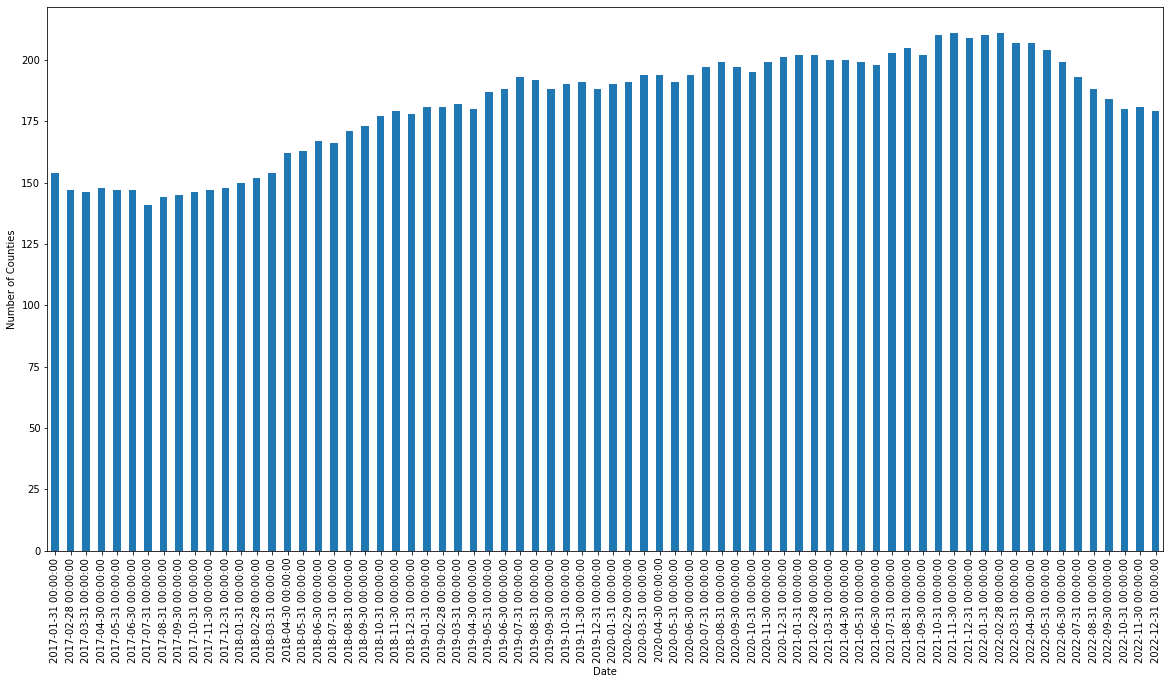
\includegraphics[width=\linewidth]{ncounties}
  \caption{Number of Counties counted over time}
\end{figure}

\begin{figure}[!htb]
  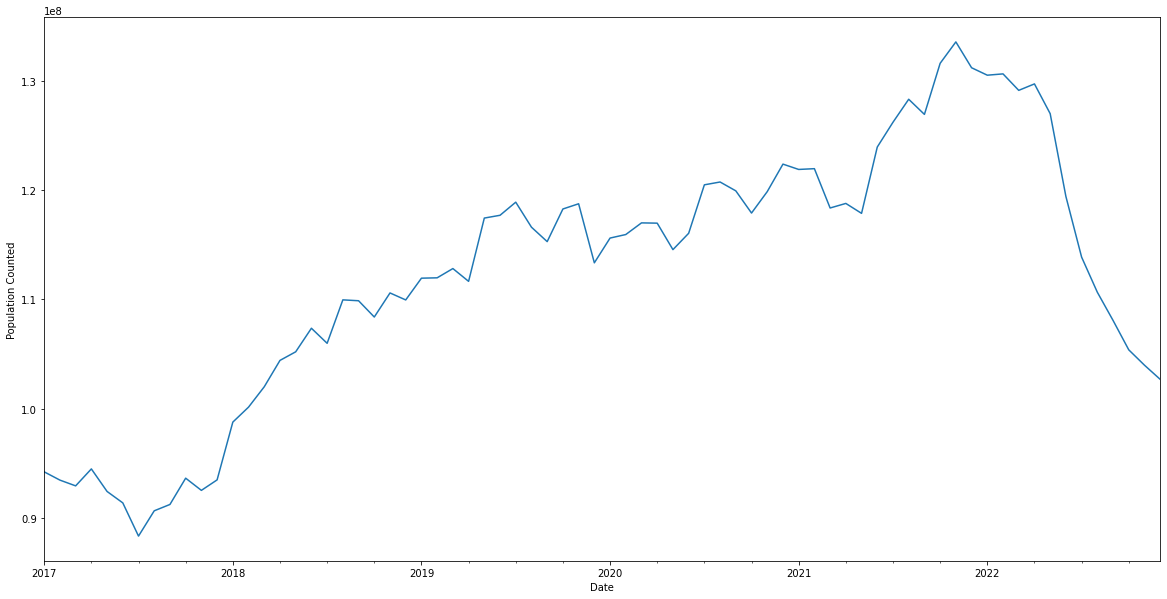
\includegraphics[width=\linewidth]{population}
  \caption{Population Counted}
\end{figure}

\begin{figure}[!htb]
  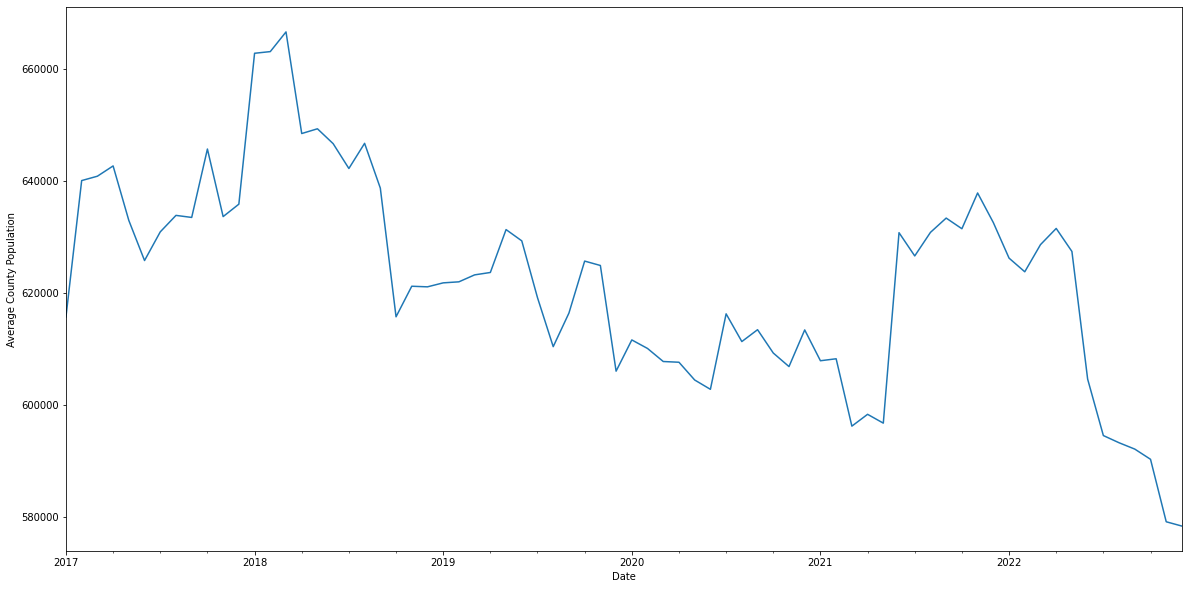
\includegraphics[width=\linewidth]{mean county population}
  \caption{Mean County Population}
\end{figure}

\begin{figure}[!htb]
  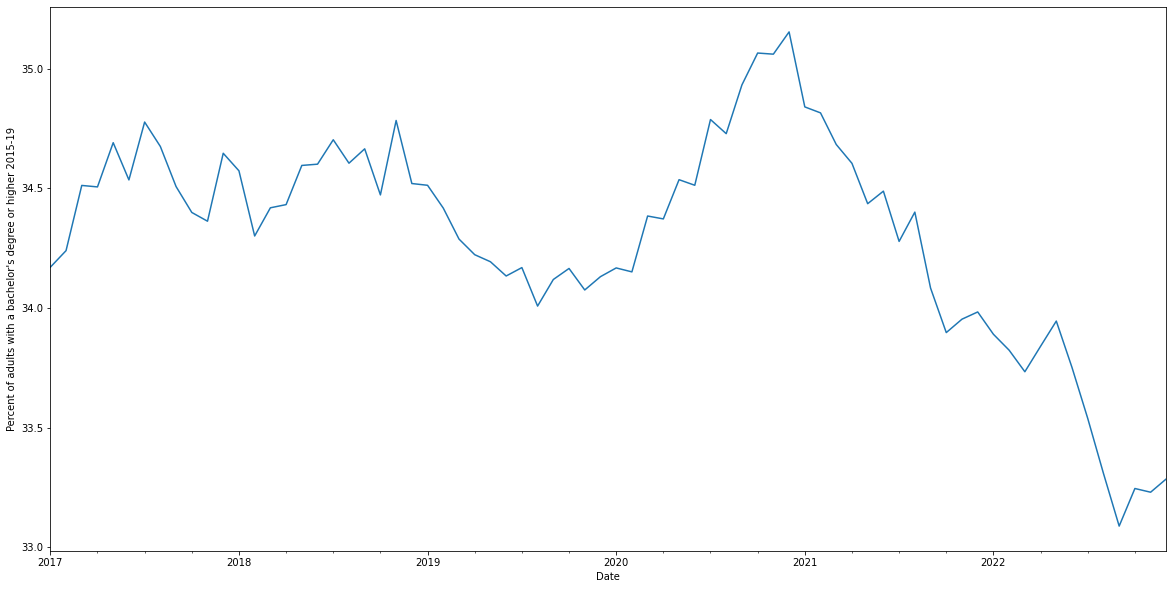
\includegraphics[width=\linewidth]{mean county educ}
  \caption{Mean County Education, Percent of Adults with a Bachelor's or Higher 2015-19}
\end{figure}

\begin{figure}[!htb]
  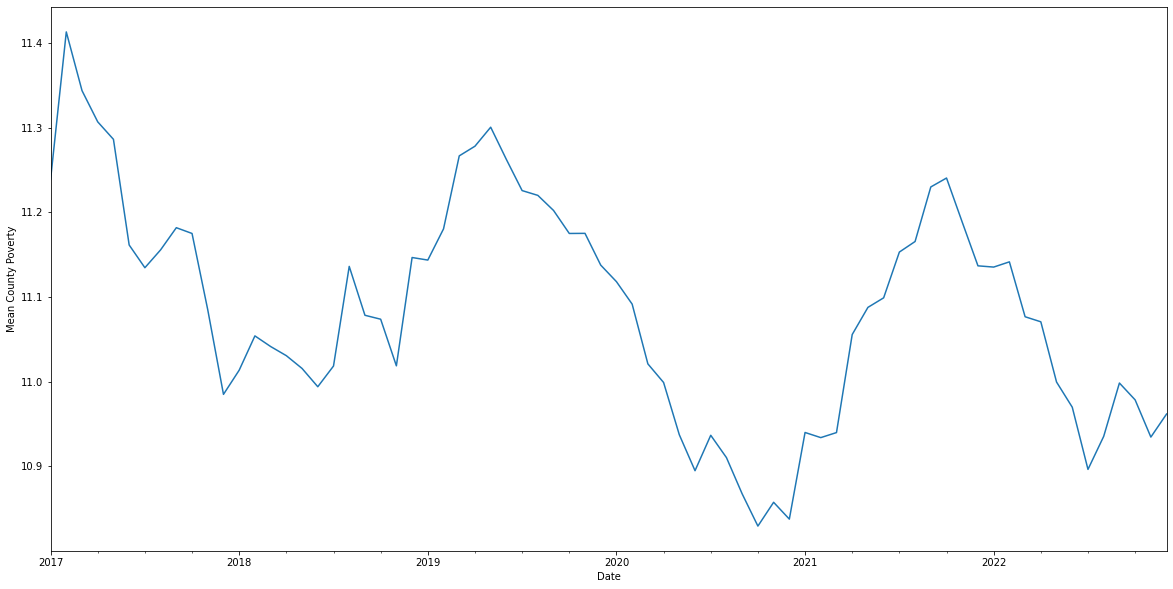
\includegraphics[width=\linewidth]{mean county pov}
  \caption{Mean County Poverty \%}
\end{figure}

\begin{figure}[!htb]
  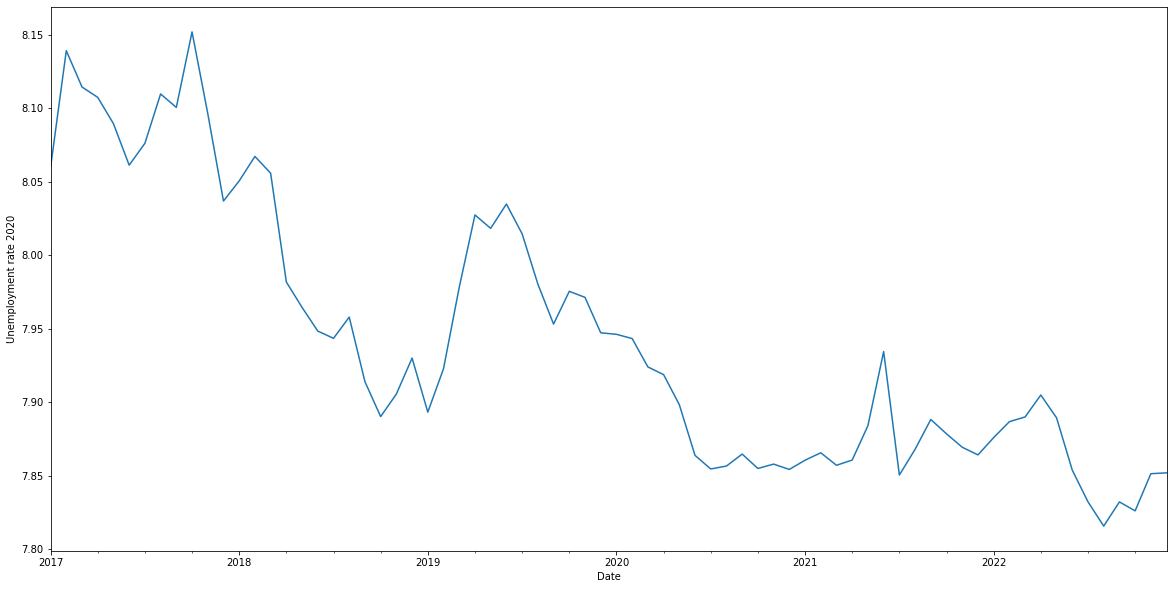
\includegraphics[width=\linewidth]{mean county unemp}
  \caption{Mean County Unemployment Rate}
\end{figure}

\begin{figure}[!htb]
  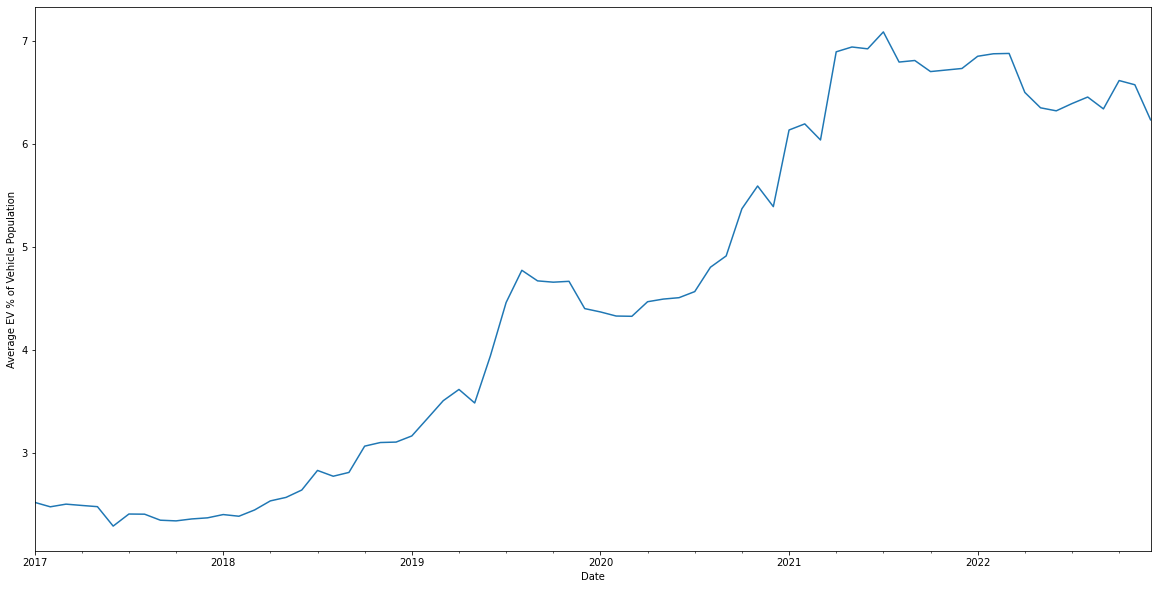
\includegraphics[width=\linewidth]{evpop}
  \caption{Average EV population as a \% of total vehicle population}
\end{figure}

\begin{figure}[!htb]
  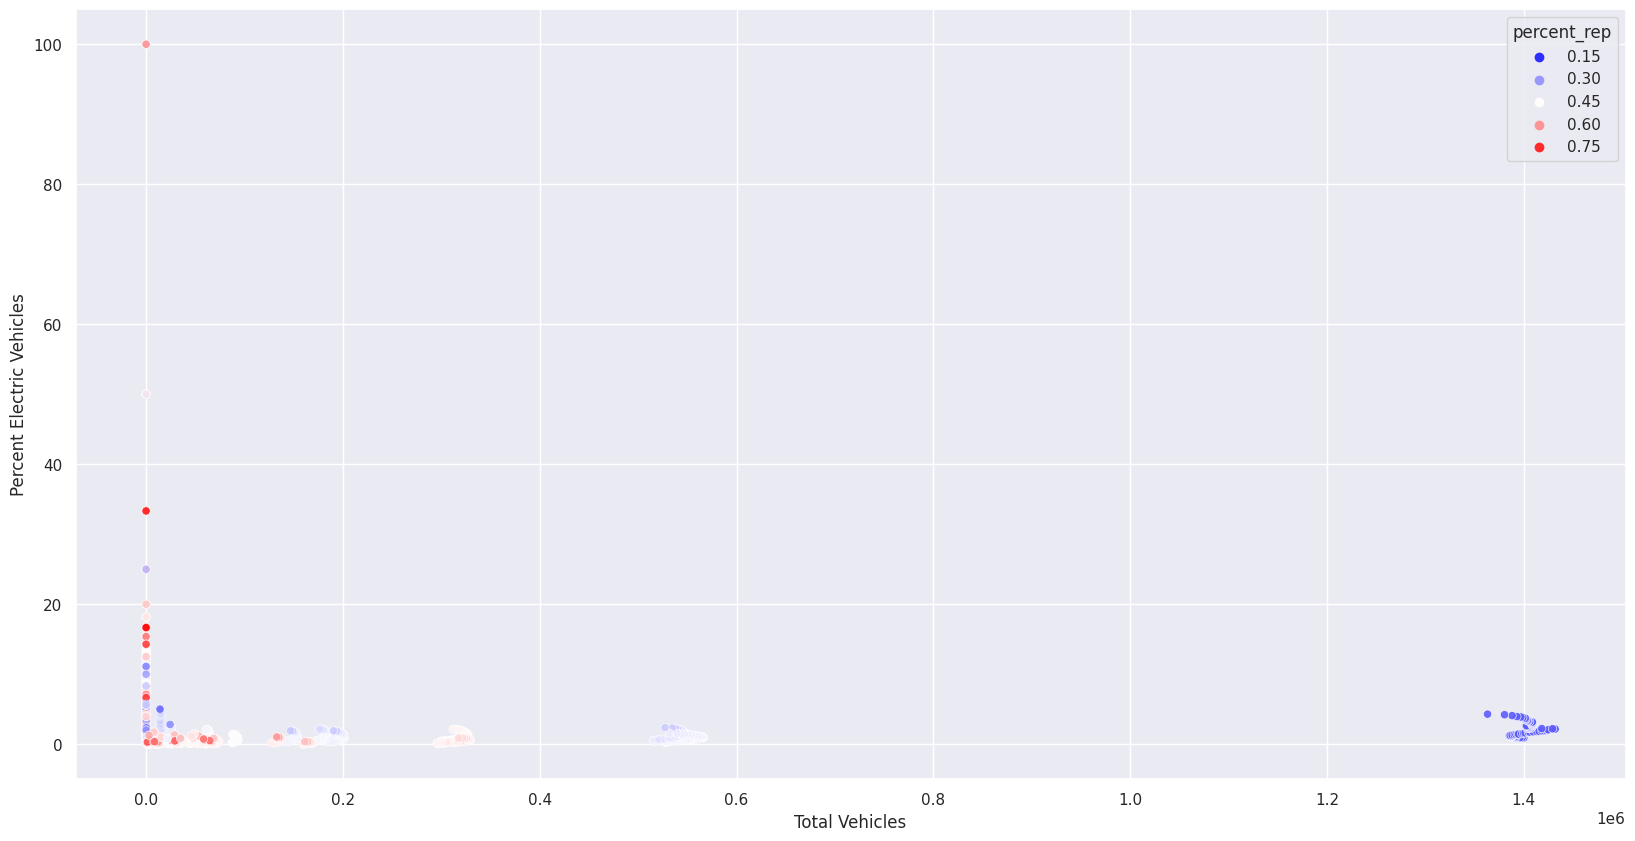
\includegraphics[width=\linewidth]{3dplot}
  \caption{Total Vehicles to EV, segmented by Republican Vote Share}
\end{figure}

\begin{figure}[!htb]
  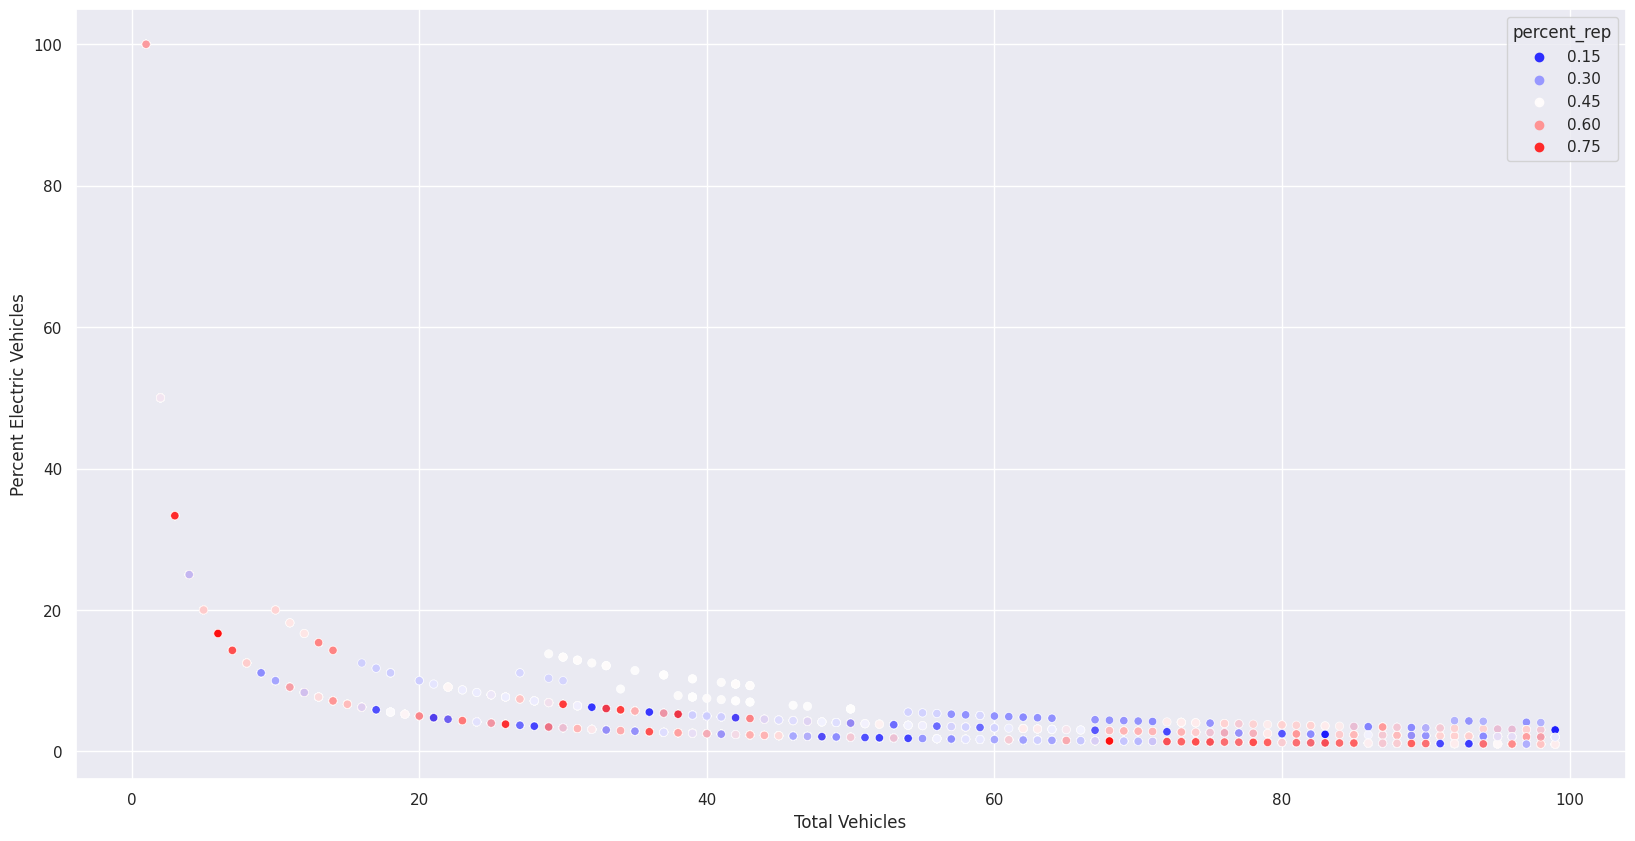
\includegraphics[width=\linewidth]{3dplot2}
  \caption{Total Vehicles to EV, segmented by Republican Vote Share, Total Vehicles $ < $ 100}
\end{figure}

\newpage

\printbibliography[
title={References}
]
\end{document}
